%%%%%%%%%%%%
\documentclass[11pt]{article}
\usepackage{latexsym}
\usepackage{amsmath}
\usepackage{graphicx}
\DeclareGraphicsExtensions{.pdf,.png,.jpg}
\usepackage[top=1in, bottom=1in, left=1in, right=1in]{geometry}


\parindent0pt
\parskip\bigskipamount

\begin{document}

\centerline{\textbf{2018 INFORMS O.R. {\&} Analytics Student Team Competition -- ENTRY FORM}}

\baselineskip16pt plus 1pt minus 1pt


\textbf{Entry Number: [}2018ORASTC252]

\textbf{Executive Summary (not to exceed 2 pages)}\\*


\textbf{Team Makeup {\&} Process}\\*

\textbf{Framing the Problem}\\*
%Rebalancing을 위한 로직 (turnover 반영)
%파라메터 $\gamma$ 반영방법?!
%Robustness


\textbf{Data}\\*
\begin{itemize}
\item[1.] The Structure of the Data %데이터 구조 및 분석
\item[] The data from Principal consists of 3 parts which are timeseries data, riskmodels data, and result template data. 
\begin{itemize}
	\item Time Series Data :
	\begin{itemize}
		\item[] 
	\end{itemize}
	\item Riskmodels Data :
	\begin{itemize}
		\item[] 
	\end{itemize}
	\item Result Template Data :
	\begin{itemize}
		\item[] 
	\end{itemize}
\end{itemize}

\item[2.] Data Pre-processing and Rescailing

	% 왜 data preprocessing이 필요한가. 어떤 방식으로 하였는가 (전반적)
	\item[ ] There are some difficulties in applying the data given from Principal directly to the model. Therefore, we present the following data preprocessing process. To make the data composed of three parts more flexible, a process of data preprocessing formed dataframe using the Pandas Library(http://pandas.pydata.org) in Python. 
	
	% Timeseries를 가지고 있는 Time Series Data 및 Result Template Data를 날짜별로 추출
	In particular, as rebalancing is carried out, it is configured to extract not all time series data, but only the data needed for the iteration. The parameters used in model were extracted from data frames formed for each period, when each parameter (Alpha Score($\alpha$), Beta($\beta$),4 Weekly Returns ($r$), etc) was set with the 'SEDOL' index as the key value. This dictionary data type is proper to consider a list of assets that may change every period.
	
	% Riskmodel Data에서 Omega(Risk Matrix)를 추출하는 방식
	The parameter Omega ($ \Omega $) is specified as the covariance matrix for a given data. In this case, the index in the columns and rows are 'SEDOL', the key value of the time series dictionary derived from the above, and are constructed in the form of full matrix. 
	
	% Quadratic 을 표현하기 위해 필요한 정제 (????)
	
	%Data Rescailing
	%\omega * \omega 와 alpha score(범위 : -2.08e-05~1.93e-05) 의 값이 너무 작음 --> Python의 한계수치로 인한 계산 오류 발생 가능성 및  Optimization Tool CPLEX에서 값이 무시되는 경우 가 생길 수 있음.
	
\item[3.] The Analysis of the Data
	% MCAPQ 와 SECTOR별 Weight의 범위 (결과?와 연관지어서)
	% Active Share과 Tracking Error의 관계 (데이터 기반)
	% 추가 historical 데이터 확보 및 분석 --> omega 도출 결과 corelation이 낮음 => 이유 간단히 분석?
	
\end{itemize}

\textbf{Methodology Approach {\&} Model Building}\\*
\begin{itemize}

\item[1.] Global Approach
	\item[] \underline{Formulation Approach }:
	% CPLEX를 가지고 QCQP 풀었을 경우 (1) Linearlize (2) Handling non-convex constraints -> Bisearch Approach (3)간단한 실험 (4)실험결과 분석 (문제를 어렵게 만드는 제약조건 , cardinality 제약식)
	Before buiding the model, we tried to solve the  Quadratic Constraint Quadratic Programming (QCQP)  problem by using the IBM CPLEX, which is well known Optmization tool, to determine the difficulty of the problem. Since CPLEX can not deal with non-linear constraints,the given formulation is required to be reformulated. 
	First, the constraints (9) are reformulated as follows:
	\begin{align*}
	\text{(9*)} \quad
	& y_i \geq w_i, \quad \forall i \in N \\
	& y_i \leq w_i + 0.999 \quad \forall i \in N \\
	& 50 \leq \sum_{i \in N} y_i \leq 70 \\
	& y_i \in \{0,1\}, \quad \forall i \in N 
	\end{align*}
	The decision variables $y_i$ is 1 if asset $i \in N$ is selected where $w_i$ is bigger than 0. Because $w_i \leq 0.001$ is considered to $w_i = 0$,  $y_i = 0$ if $w_i = 0$. The opposite is the same as well. Constraints (10) and (11) are also non-linear. Furthermore, if non-convex constraints are linearized, they significantly impact speed by increasing the number of variables to determine and the number of constraints to consider. In other words, it is very inefficient to reformulate Constraints (10) and (11), which represent the limits of Active Share and Tracking Error, respectively. Therefore, we propose a bisearch algorithm to adjust Active share and Tracking Error.
	
	%bisearch algorithm 내용
	
	\item[]\underline{Evolutionary Approach} :
	
	% 진화 알고리즘 (ex.EDA)으로 접근. (간단한 실험?) -> 문제점 도출 : population의 수를 크게 두고 여러번 풀어 확률적 이론 등을 적용시키는 데에는 오랜시간 소요.
	
	\item[]\underline{Neural Network Approach} :
	
	% DeepLearning 기법을 이용함 -> 세밀한 수치을 조정하기 위해서는 training 시간이 오래걸릴 뿐만 아니라 모든 제약식에 대해 feasible한 set을 찾기에는 무리가 있음. 
	
	
\item[2.] Hybrid Approach %이름

When solving the problem with the formulation appraoch, we could not find a reasonable solution because to consider about 500 assets per iteration the number of decision variables to decide and the number of constraints to be satisfied are too high . Especially, constraints (9) which select cardinalities considering the target range on number of stocks make the problem difficult. 
% 진화알고리즘의 단점 추가
In the case of Neural Network Approach, there is a great advantage in that a solution that does not get significantly out from the whole constraints and that has a good objective value can be considered at the same time. However, it is difficult to find a soluton satisfying the feasibility for all the constraints and the fact that the training time takes too much time.

\begin{figure}[h] 
	\begin{center}
		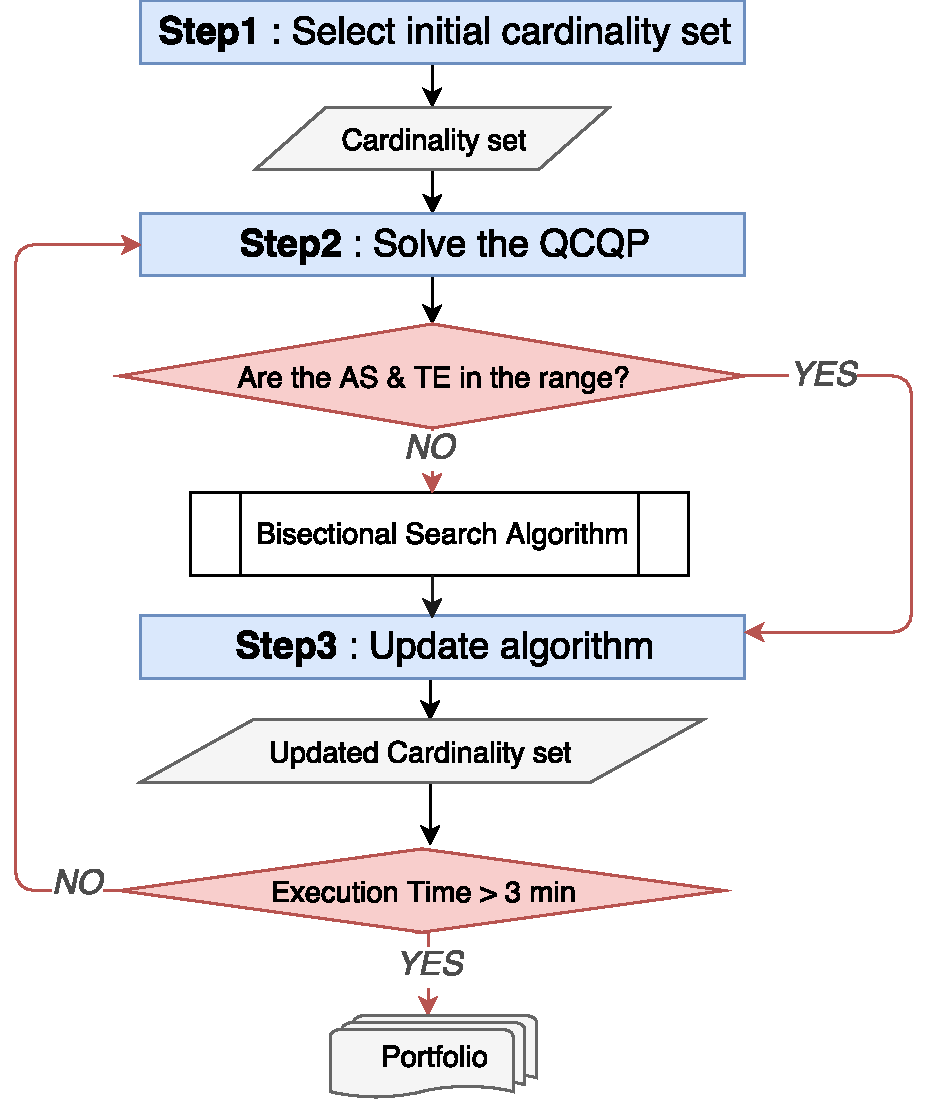
\includegraphics[width=0.45\textwidth]{flowchart}
		\caption{A flowchart of ...} \label{fig:flowchart}
	\end{center}
\end{figure}
	
	- 제시하는 모델의 전체적인 구조 제시 (Flow Chart)
	1) initial cardinality set 지정 : 
	- optimal solution을 도출하는 최적화 기법인 B&B algorithm을 이용했을때, tab1과 같이 cardinality 선택에서 어려움이 있으므로 이를 해소시키기 위한 방도. 
	- objective value(Return 대비 Risk) 가 낮아지는 좋은 cardinality set 을 찾아보자!
	- 3가지 방법(Random, Cplex, GAN)을 제시
	- 각 방법의 원리 설명
	
	
	2) 1)로부터 얻어진 cardinality set을 Cplex 수리모형에 적용 
	- 실험 결과 및 정리 (Tab2)
	
	3) 초기 해 개선 알고리즘
	
	4) Turnover 계산 후 다음 기간(date)에 반영
	
	
	- Robustness고려
	


\end{itemize}
\textbf{Analytics Solution and Results}\\*




\begin{itemize}
\item \underline {This Entry Form}: Present your solution and results in this section, including completion of the Portfolio Performance Statistics chart below. You may supplement your analysis with additional charts, diagrams and/or other visualization; these supplements must be incorporated into this section of the Entry From.
\end{itemize}

\begin{center}
\textbf{Portfolio Performance Statistics}\vspace*{-14pt}
\end{center}
\begin{table}[htbp]
\def\arraystretch{1.4}
\begin{center}
\begin{tabular}{|l|c|c|}
\hline
\textbf{2007-01-01 to 2016-12-31}& 
\textbf{Portfolio}& 
\textbf{Benchmark} \\
\hline
Cumulative Return& 
{\%}& 
{\%} \\
\hline
Annualized Return& 
{\%}& 
{\%} \\
\hline
Annualized Excess Return& 
{\%}& 
-- \\
\hline
Annualized Tracking Error& 
{\%}& 
-- \\
\hline
Sharpe Ratio& 
& 
 \\
\hline
Information Ratio& 
& 
-- \\
\hline
\end{tabular}
\label{tab1}
\end{center}
\end{table}

\begin{itemize}
\item \underline {Results Template}: Populate and submit your numerical results using the Results Template. This template is provided as a separate file on the Competition download site. You can use either the Excel or CSV version.
\end{itemize}

\textbf{References}

\bgroup
\parskip0pt

Please follow guidelines in the \textit{Chicago Manual of Style,} 16$^{\text{th}}$ Edition. Here are examples: 

\begin{itemize}
\item[--] Journal article: Flynn J, Gartska SK (1990) A dynamic inventory model with periodic auditing. \textit{Oper. Res.} 38(6):1089--1103. 
\item[--] Book: Makridakis S, Wheelwright SC, McGee VE (1983) \textit{Forecasting: Methods and Applications}, 2nd ed. (John Wiley {\&} Sons, New York). 
\item[--] Edited Book: Martello S, Toth P (1979) The 0-1 knapsack problem. Christofides N, Mingozzi A, Sandi C, eds. \textit{Combinatorial Optimization} (John Wiley {\&} Sons, New York), 237--279.
\item[--] Online reference, fictional example: American Mathematical Institute (2005) Better predictors of geospatial variability. Retrieved June 14, 2005, \underline {www.mathematicsinstitute}.

\end{itemize}

\egroup

\end{document}
